% -*- latex -*-
%
% Copyright (c) 2002 The Trustees of Indiana University.  
%                    All rights reserved.
% 
% This file is part of the OSCAR software package.  For license
% information, see the COPYING file in the top level directory of the
% OSCAR source distribution.
%
% $Id: screen-by-screen.tex,v 1.19 2002/11/17 04:02:40 jsquyres Exp $
%
% $COPYRIGHT$
%

%% Put ourselves on a new page because we go and change the margins for
%% our images
\newpage

\section{Screen-by-Screen Walkthrough}
\label{app:screen-by-screen}

The following is a screen-by-screen walkthrough of a simple installation.
It is intended as supplementary material to aid in providing a better feel
for the general progression of the installation.  For a detailed discussion
of the steps, please refer to the Detailed Cluster Installation Procedure. 

Note the example screen shots were based in a Red Hat 7.3 using a
pre-release version of OSCAR \oscarversion\ in the KDE graphical
environment.  Since this section is intended as a supplementary source
of information, it is judged to be ``close enough'' to the real
\oscarversion\ release.  Just beware that some of the screenshots may
not be {\em exactly} what you see in the \oscarversion\ release.

Also note that these images have been scaled down to fit within the
document.  As such, although they are readable, the images may not
render nicely on a screen.  The images tend be much more readable on
an actual printout.


%------------------------------------------------------------------
% Running install_cluster
%------------------------------------------------------------------

\subsection{Running \cmd{install\_cluster}}

This step comprises of running the \cmd{install\_cluster} script with
the network interface name.  See details in
Section~\ref{det:installcluster}, page~\pageref{det:installcluster}.

% JMS: These images were captured using KDE ``konsole'' tools, with
% the ``small'' font, using a black-on-white schema, and resized to be
% 80x26.

\begin{figure}[h!]
  \begin{center}
    \centerline{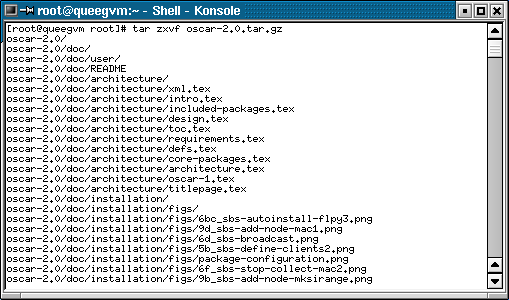
\includegraphics[scale=\imgscale]{figs/0c_sbs-unpack}}
    \caption{Unpacking OSCAR.}
    \label{fig:sbs-unpacking-oscar}
  \end{center}
\end{figure}

\begin{figure}[h!]
  \begin{center}
    \centerline{
      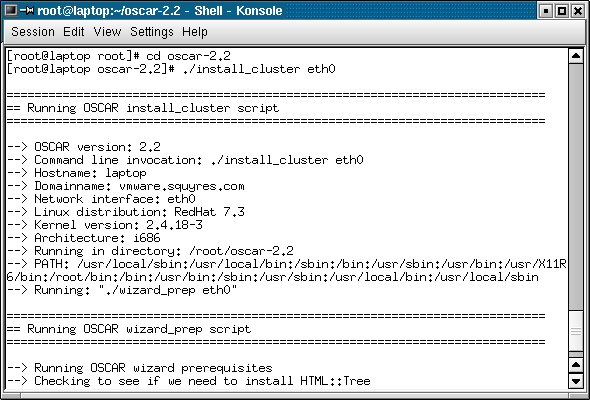
\includegraphics[scale=\imgscale]{figs/1a_sbs-install-oscar}
      \hspace{\imghskip}
      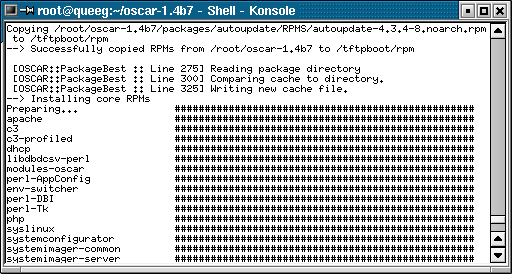
\includegraphics[scale=\imgscale]{figs/1b_sbs-install-oscar2}
      }
    \caption{Running the \cmd{install\_cluster} script.}
    \label{fig:sbs-install-oscar}
  \end{center}
\end{figure}

\begin{figure}[ht!]
  \begin{center}
    \centerline{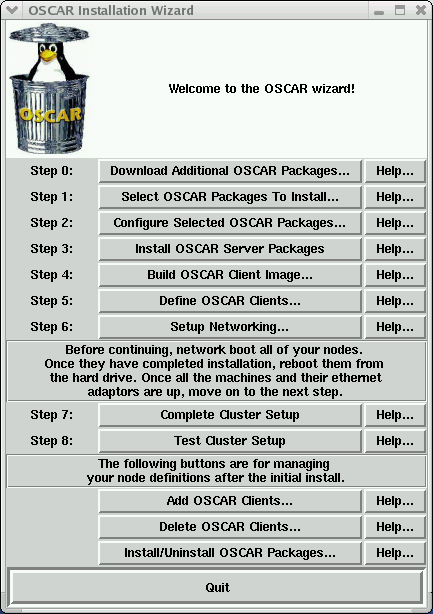
\includegraphics[scale=\imgscale]{figs/2_sbs-oscar-wizard}}
    \caption{The OSCAR Installation Wizard.}
    \label{fig:sbs-install-wizard}
  \end{center}
\end{figure}


%------------------------------------------------------------------
% Step 1: Prepare OSCAR Server For Install
%------------------------------------------------------------------

\subsection{Step 1: Prepare OSCAR Server for Install}

Step 1 is used to setup the server for the OSCAR cluster.  See details
in Section~\ref{det:prepareforinstall},
page~\pageref{det:prepareforinstall}. 

\begin{figure}[hb!]
  \begin{center}
    \centerline{
      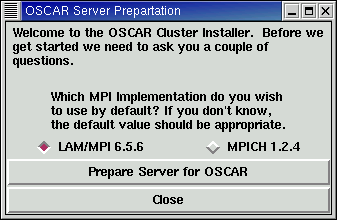
\includegraphics[scale=\imgscale]{figs/3a_sbs-wizard-step1}
      \hspace{\imghskip}
      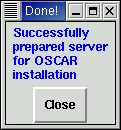
\includegraphics[scale=\imgscale]{figs/3b_sbs-wizard-step1}
      }
    \caption{Step 1 -- Select default MPI implementation and prepare server.}
    \label{fig:sbs-install-wizard-s1}
  \end{center}
\end{figure}


%------------------------------------------------------------------
% Step 2: Build OSCAR Client Image
%------------------------------------------------------------------

\subsection{Step 2: Build OSCAR Client Image}

Step 2 builds a disk image for the clients to download and install
onto their local disks.  See the details in
Section~\ref{det:buildimage}, page~\pageref{det:buildimage}.

\begin{figure}[h!]
  \begin{center}
    \centerline{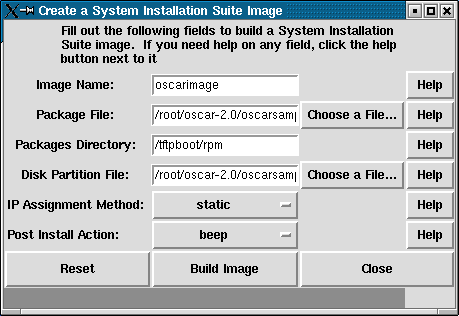
\includegraphics[scale=\imgscale]{figs/4a_sbs-build-image1}}
    \vspace{\imgvskip}
    \centerline{
      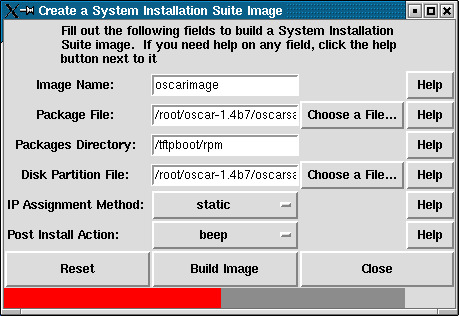
\includegraphics[scale=\imgscale]{figs/4b_sbs-build-image2}
      \hspace{\imghskip}
      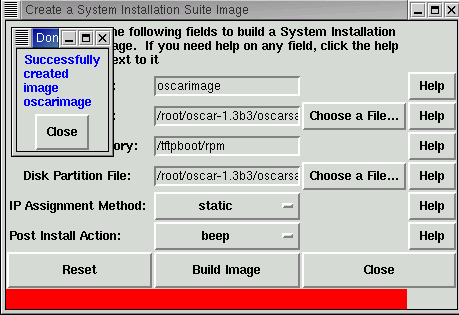
\includegraphics[scale=\imgscale]{figs/4c_sbs-build-image3}
      }
    \caption{Step 2 -- Building the image.}
    \label{fig:sbs-build-image}
  \end{center}
\end{figure}


%------------------------------------------------------------------
% Step 3: Define OSCAR Clients
%------------------------------------------------------------------

\clearpage
\subsection{Step 3: Define OSCAR Clients}

Step 3 is used to specify how many clients there will be, and what
their TCP/IP characteristics will be.  See the details in
Section~\ref{det:defclients}, page~\pageref{det:defclients}.
 
\begin{figure}[ht!]
  \begin{center}
    \centerline{
      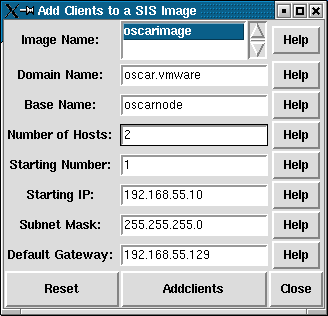
\includegraphics[scale=\imgscale]{figs/5a_sbs-define-clients1}
      \hspace{\imghskip}
      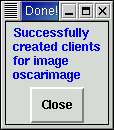
\includegraphics[scale=\imgscale]{figs/5b_sbs-define-clients2}
      }
    \caption{Step 3 -- Defining the clients.}
    \label{fig:sbs-define-clients}
  \end{center}
\end{figure}


%------------------------------------------------------------------
% Step 4: Setup Networking
%------------------------------------------------------------------

\subsection{Step 4: Setup Networking}

Step 4 is used to collect the MAC addresses of the clients, and then
download the disk images to the clients.  See the details in
Section~\ref{det:setupnetwork}, page~\pageref{det:setupnetwork}.

\begin{figure}[h!]
  \begin{center}
    \centerline{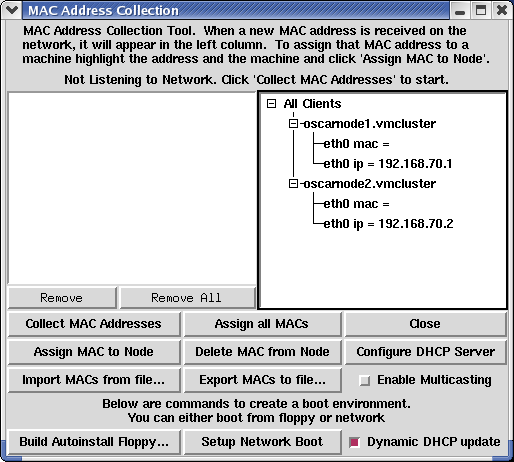
\includegraphics[scale=\imgscale]{figs/6a_sbs-collect-mac1}}
    \caption{Beginning step 4 -- Setting up networking.}
    \label{fig:sbs-setup-network1}
  \end{center}
\end{figure}

%-------
% Show how to create the boot floppy
%-------

\begin{figure}[h!]
  \begin{center}
    \centerline{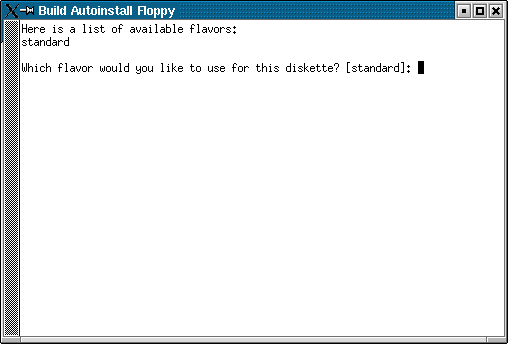
\includegraphics[scale=\imgscale]{figs/6ba_sbs-autoinstall-flpy1}}
    \vspace{\imgvskip}
    \centerline{
      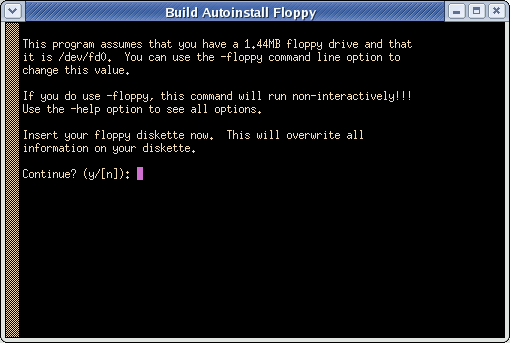
\includegraphics[scale=\imgscale]{figs/6bb_sbs-autoinstall-flpy2}
      \hspace{\imghskip}
      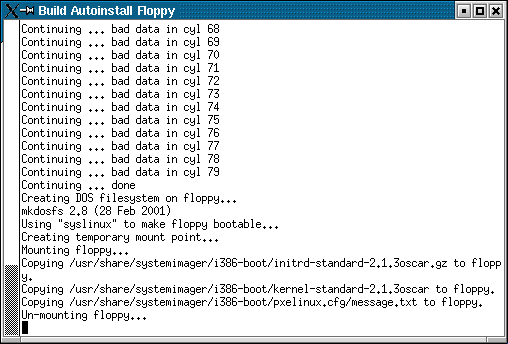
\includegraphics[scale=\imgscale]{figs/6bc_sbs-autoinstall-flpy3}
      }
    \caption{Further progress in step 4 -- Build Autoinstall Floppy.}
    \label{fig:sbs-autoinstall-flpy1}
  \end{center}
\end{figure}

%-------
% Booting the client
%-------

\begin{figure}[h!]
  \begin{center}
    \centerline{
      \framebox{
        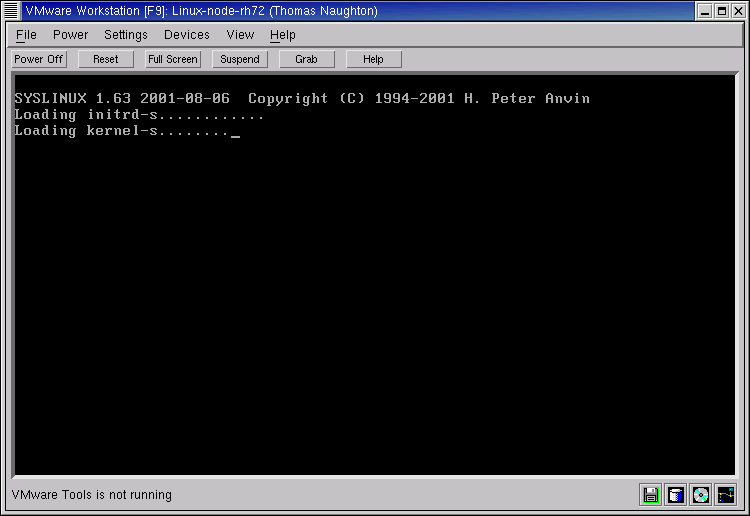
\includegraphics[scale=\imgscale]{figs/6c_sbs-client-boot1}
        }
      }
    \caption{Further progress in step 4 -- Booting the client.}
    \label{fig:sbs-collect-boot1}
  \end{center}
\end{figure}

\begin{figure}[h!]
  \begin{center}
    \centerline{
      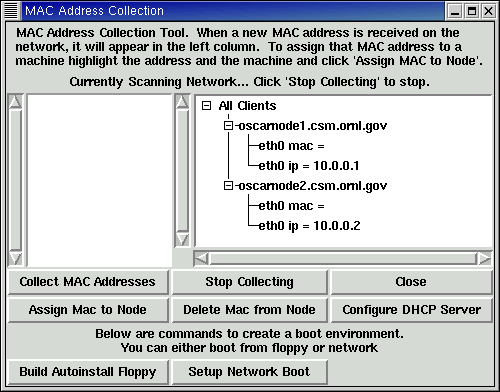
\includegraphics[scale=\imgscale]{figs/6ca_sbs-client-boot1}}
    \caption{Further progress in step 4 -- Scan for booting client (DHCP
      request).}
    \label{fig:sbs-client-boot2}
  \end{center}
\end{figure}

\begin{figure}[h!]
  \begin{center}
    \centerline{
      \framebox{
        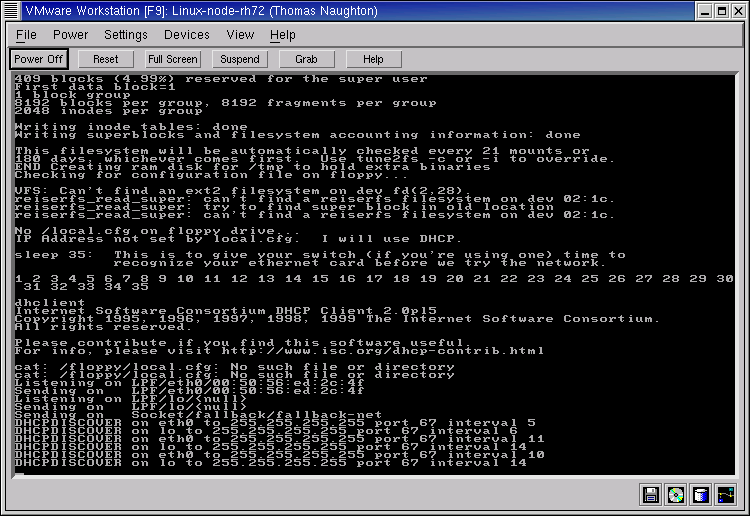
\includegraphics[scale=\imgscale]{figs/6d_sbs-broadcast}
        }
      }
    \caption{Further progress in step 4 -- Client is broadcasting, in
      order to acquire MAC address.}
    \label{fig:sbs-collect-broadcast} 
  \end{center}
\end{figure}

\begin{figure}[h!]
  \begin{center}
    \centerline{
      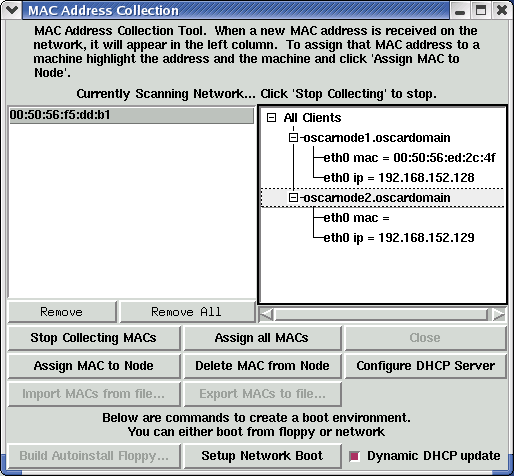
\includegraphics[scale=\imgscale]{figs/6e_sbs-found-mac}
      \hspace{\imghskip}
      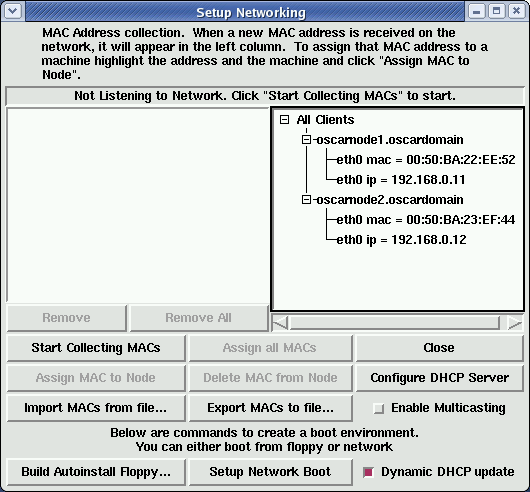
\includegraphics[scale=\imgscale]{figs/6f_sbs-stop-collect-mac2}
      }
    \caption[Further progress in step 4 -- Assigning MACs to
      IPs]{Further progress in step 4 -- Scanning network, found first
        MAC address, then later assigned all MAC addresses.}
    \label{fig:sbs-setup-network2}
  \end{center}
\end{figure}

%-------
% Client downloading and installing the image
%-------

\begin{figure}[h!]
  \begin{center}
    \centerline{
      \framebox{
        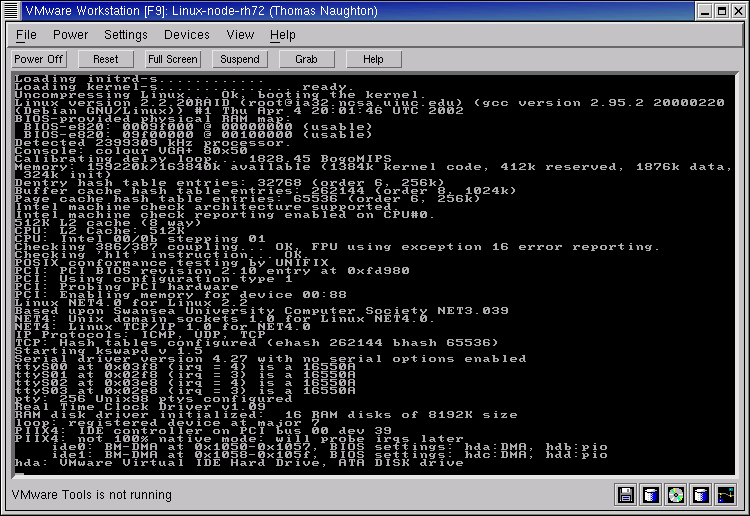
\includegraphics[scale=\imgscale]{figs/6h_sbs-client-boot}
        }
      }
    \caption{Booting the client a second time to download the image.}
    \label{fig:sbs-install-boot}
  \end{center}
\end{figure}

\begin{figure}[h!]
  \begin{center}
    \centerline{
      \framebox{
        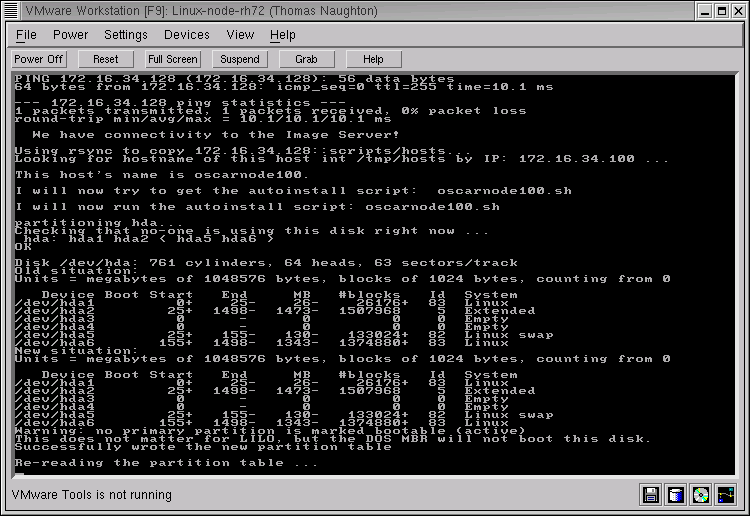
\includegraphics[scale=\imgscale]{figs/6i_sbs-client-diskpar}
        }
      }
    \caption{Client partitioning disk, setting up the disk tables, and
      starting to download the image.}
    \label{fig:sbs-install-diskpar}
  \end{center}
\end{figure}
  
\begin{figure}[h!]
  \begin{center}
    \centerline{
      \framebox{
        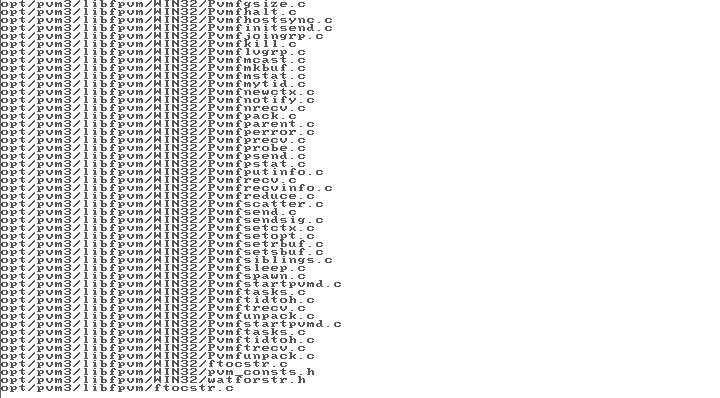
\includegraphics[scale=\imgscale]{figs/6j_sbs-client-rsync}
        }
      }
    \caption{Client downloading and installing the image.}
    \label{fig:sbs-install-rsync}
  \end{center}
\end{figure}

\begin{figure}[h!]
  \begin{center}
    \centerline{
      \framebox{
        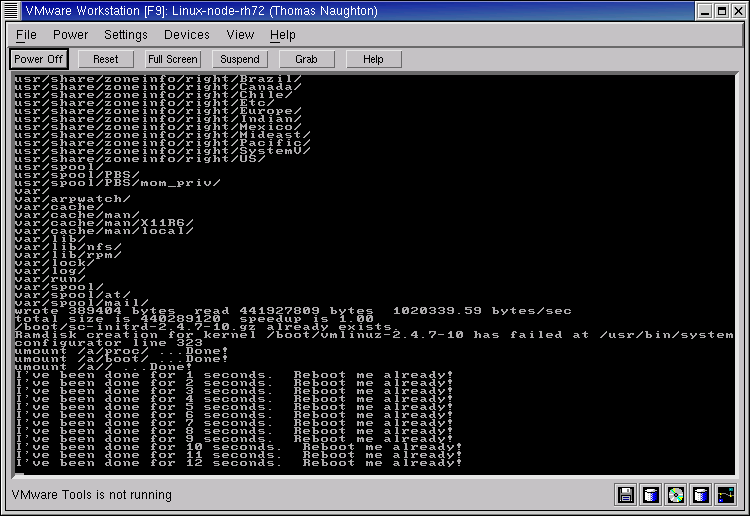
\includegraphics[scale=\imgscale]{figs/6k_sbs-rebootme}
        }
      }
    \caption{A client has finished the install and is asking to be
      rebooted.} 
    \label{fig:sbs-install-finish}
  \end{center}
\end{figure}


%------------------------------------------------------------------
% Step 5: Complete Cluster Install
%------------------------------------------------------------------

\clearpage
\subsection{Step 5: Complete Cluster Install} 

Step 5 is used to unify the server and client installations into a
single cluster.  See the details in
Section~\ref{det:complete-cluster-setup},
page~\pageref{det:complete-cluster-setup}.

\begin{figure}[h!]
   \begin{center}
     \centerline{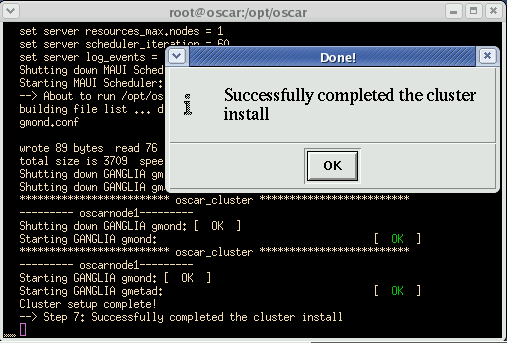
\includegraphics[scale=\imgscale]{figs/7_sbs-complete-cluster-setup}}
     \caption{Step 5 -- Complete Cluster Setup.}
     \label{fig:sbs-install-wizard-s5}
   \end{center}
 \end{figure}


%------------------------------------------------------------------
% Step 6: Test Cluster Setup
%------------------------------------------------------------------

\subsection{Step 6: Test Cluster Setup}

Step 6 is used to test the cluster setup.  It can either be run from
within the wizard, or, as shown here, from manually launching a shell
script at a \user{root} command prompt.  See the details in
Section~\ref{det:test-cluster}, page~\pageref{det:test-cluster}.

\begin{figure}[h!]
  \begin{center}
    \centerline{
      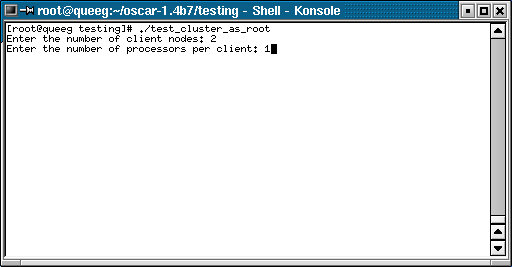
\includegraphics[scale=\imgscale]{figs/8_sbs-test-cluster-prompt}
      \hspace{\imghskip}
      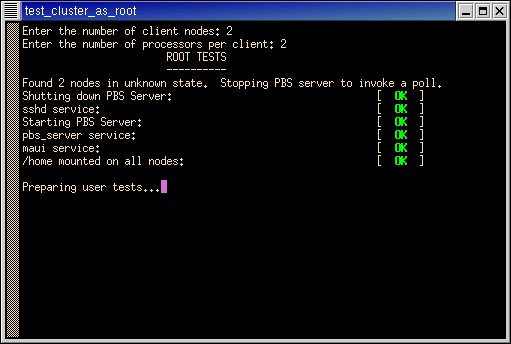
\includegraphics[scale=\imgscale]{figs/8_sbs-test-cluster-root-tests}
      }
    \vspace{\imgvskip}
    \centerline{
      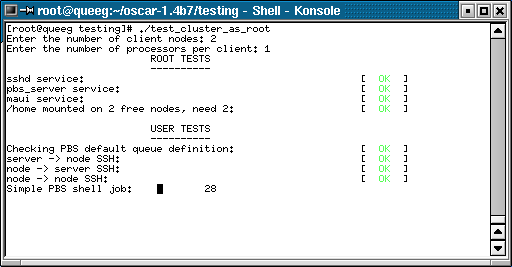
\includegraphics[scale=\imgscale]{figs/8_sbs-test-cluster-user-tests}
      \hspace{\imghskip}
      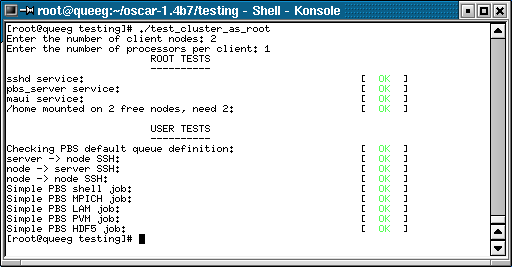
\includegraphics[scale=\imgscale]{figs/8_test-cluster-complete}
      }
    \caption{Step 6 -- Test the cluster.}
    \label{fig:sbs-setup-test}
  \end{center}
\end{figure}


%-----------------------------------------------------------------
% Delete Node Button
%-----------------------------------------------------------------

\subsection{Delete Node Button}
\label{app:sbs-delete-node}

The Delete Node button can be used to delete clients from an OSCAR
cluster.  Note that this button only deletes OSCAR's knowledge of the
clients -- what physically happens to that client is not OSCAR's
concern.  This example shows deleting one of the clients setup in the
previous sections -- \hostname{oscarnode2}.  The next section
(Section~\ref{app:sbs-add-node}) will show adding it back.  See the
details on deleting clients in Section~\ref{det:deleting-clients},
page~\pageref{det:deleting-clients}.

\begin{figure}[h!]
  \begin{center}
    \centerline{
      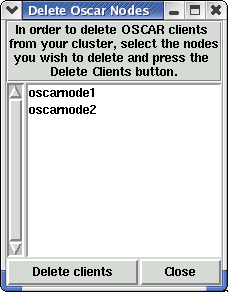
\includegraphics[scale=\imgscale]{figs/10a_sbs-del-node}
      \hspace{\imghskip}
      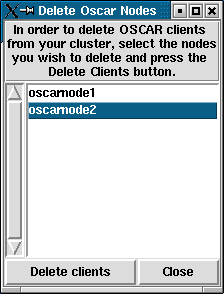
\includegraphics[scale=\imgscale]{figs/10b_sbs-del-node-partA}
      \hspace{\imghskip}
      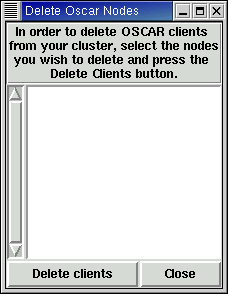
\includegraphics[scale=\imgscale]{figs/10b_sbs-del-node-partB}
      }
    \caption[Delete OSCAR Clients.]{Delete OSCAR clients.  First image
    is the initial window, second image is with a client selected, and
    third image is when the action has completed.}
    \label{fig:sbs-del-node1}
  \end{center}
\end{figure}


%------------------------------------------------------------------
% Add Node Button
%------------------------------------------------------------------

\subsection{Add Node Button}
\label{app:sbs-add-node}

The Add Node button will add clients into an existing OSCAR cluster.
In this example, we will add back \hostname{oscarnode2} into the
cluster.  See the details of adding a client in
Section~\ref{det:adding-clients}, page~\pageref{det:adding-clients}.

\begin{figure}[h!]
  \begin{center}
    \centerline{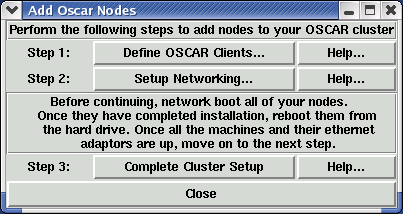
\includegraphics[scale=\imgscale]{figs/9a_sbs-add-node}}
    \caption{Add OSCAR Clients.}
    \label{fig:sbs-add-node1}
  \end{center}
\end{figure}

\begin{figure}[h!]
  \begin{center}
    \centerline{
      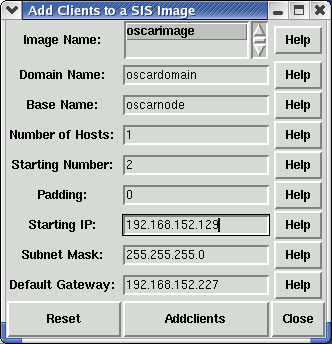
\includegraphics[scale=\imgscale]{figs/9b_sbs-add-node-mksirange}
      \hspace{\imghskip}
      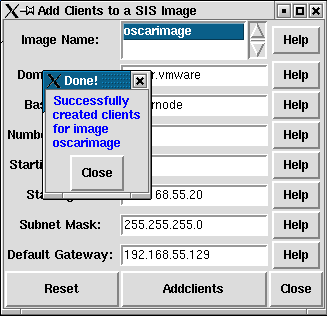
\includegraphics[scale=\imgscale]{figs/9c_sbs-add-node-success}
      }
    \caption[Add Node step 1 -- Defining the clients.]{Add Node step 1
      -- Defining the clients.  Note that you only define {\em new}
      clients here (i.e., change the starting number, starting IP,
      etc.).}
    \label{fig:sbs-add-node1-define-clients}
  \end{center}
\end{figure}

\begin{figure}[h!]
  \begin{center}
    \centerline{
      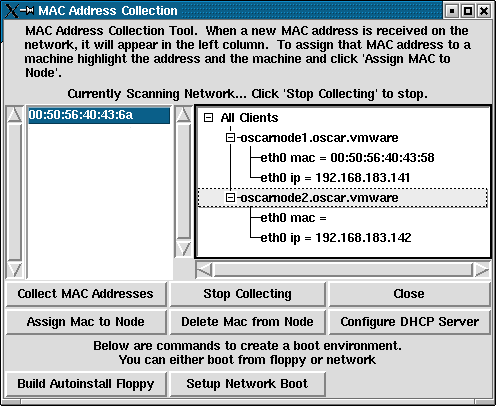
\includegraphics[scale=\imgscale]{figs/9d_sbs-add-node-mac1}
      \hspace{\imghskip}
      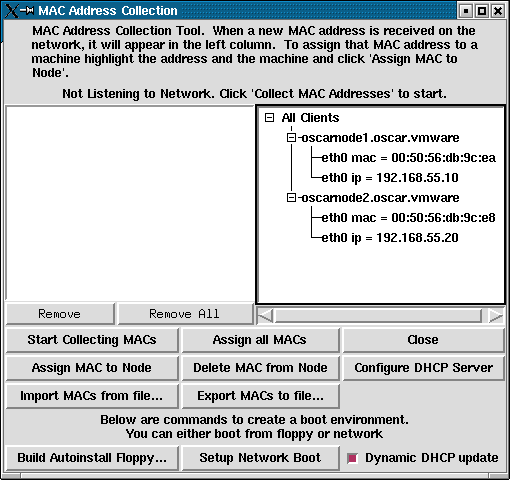
\includegraphics[scale=\imgscale]{figs/9e_sbs-add-node-mac2}
      }
    \caption{Add Node step 2 -- Setting up networking for new client(s).}
    \label{fig:sbs-add-node1-setup-network}
  \end{center}
\end{figure}

\begin{figure}[h!]
  \begin{center}
    \centerline{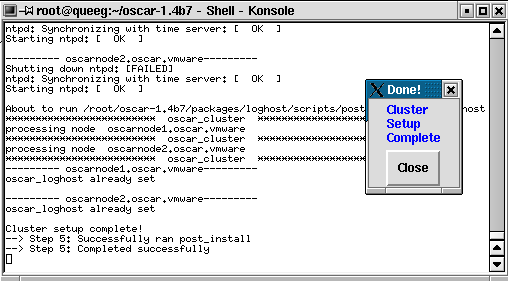
\includegraphics[scale=\imgscale]{figs/9f_sbs-add-node-complete}}
    \caption{Add Node step 3 -- Complete Cluster Setup.}
    \label{fig:sbs-add-node1-cluster-setup}
  \end{center}
\end{figure}

% LocalWords:  tex Exp sbs
